%%%%%%%%%%%%%%%%%%%%%%%%%%%%%%%%%%%%%%%%%%%%%%%%%%%%%%%%%%%%%%%%%%%%%%%%%%%%%
%% Original default rstudio/pandoc latex file
%% upated by @jhollist 09/15/2014
%% inspired by @cboetting https://github.com/cboettig/template and
%% @rmflight blog posts:
%% http://rmflight.github.io/posts/2014/07/analyses_as_packages.html 
%% http://rmflight.github.io/posts/2014/07/vignetteAnalysis.html).  
%%%%%%%%%%%%%%%%%%%%%%%%%%%%%%%%%%%%%%%%%%%%%%%%%%%%%%%%%%%%%%%%%%%%%%%%%%%%%

\documentclass[11pt,]{article}
\usepackage[T1]{fontenc}
\usepackage{lmodern}
\usepackage{amssymb,amsmath}
\usepackage{ifxetex,ifluatex}
\usepackage{fixltx2e} % provides \textsubscript
% use upquote if available, for straight quotes in verbatim environments
\IfFileExists{upquote.sty}{\usepackage{upquote}}{}
\ifnum 0\ifxetex 1\fi\ifluatex 1\fi=0 % if pdftex
  \usepackage[utf8]{inputenc}
\else % if luatex or xelatex
  \ifxetex
    \usepackage{mathspec}
    \usepackage{xltxtra,xunicode}
  \else
    \usepackage{fontspec}
  \fi
  \defaultfontfeatures{Mapping=tex-text,Scale=MatchLowercase}
  \newcommand{\euro}{€}
\fi
% use microtype if available
\IfFileExists{microtype.sty}{\usepackage{microtype}}{}
\usepackage{longtable,booktabs}
\usepackage{graphicx}
% Redefine \includegraphics so that, unless explicit options are
% given, the image width will not exceed the width of the page.
% Images get their normal width if they fit onto the page, but
% are scaled down if they would overflow the margins.
\makeatletter
\def\ScaleIfNeeded{%
  \ifdim\Gin@nat@width>\linewidth
    \linewidth
  \else
    \Gin@nat@width
  \fi
}
\makeatother
\let\Oldincludegraphics\includegraphics
{%
 \catcode`\@=11\relax%
 \gdef\includegraphics{\@ifnextchar[{\Oldincludegraphics}{\Oldincludegraphics[width=\ScaleIfNeeded]}}%
}%
\ifxetex
  \usepackage[setpagesize=false, % page size defined by xetex
              unicode=false, % unicode breaks when used with xetex
              xetex]{hyperref}
\else
  \usepackage[unicode=true]{hyperref}
\fi
\hypersetup{breaklinks=true,
            bookmarks=true,
            pdfauthor={},
            pdftitle={Modeling Lake Trophic State: A Data Mining Approach},
            colorlinks=true,
            citecolor=blue,
            urlcolor=blue,
            linkcolor=magenta,
            pdfborder={0 0 0}}
\urlstyle{same}  % don't use monospace font for urls
\setlength{\parindent}{0pt}
\setlength{\parskip}{6pt plus 2pt minus 1pt}
\setlength{\emergencystretch}{3em}  % prevent overfull lines
\setcounter{secnumdepth}{5}

%%%%%%%%%%%%%%%%%%%%%%%%%%%%%%%%%%%%%%%%%%%%%%%%%%%%%%%%
%Changes borrowed from @cboettig, added by @jhollist 
% A modified page layout 
\textwidth 6.75in
\oddsidemargin -0.15in
\evensidemargin -0.15in
\textheight 9in
\topmargin -0.5in
\usepackage{lineno} % add 
%%%%%%%%%%%%%%%%%%%%%%%%%%%%%%%%%%%%%%%%%%%%%%%%%%%%%%%%

%%%%%%%%%%%%%%%%%%%%%%%%%%%%%%%%%%%%%%%%%%%%%%%%%%%%%%%%
%%Packages and layout changes by @jhollist 09/15/2014
\usepackage{ragged2e}
\usepackage[font=normalsize]{caption}
  \usepackage[onehalfspacing]{setspace}
\usepackage{parskip}
\usepackage{fancyhdr}
\pagestyle{fancy}
\fancyhf{}
\renewcommand{\headrulewidth}{0pt}
\rfoot{\today}
\lfoot{\thepage}
%%Changed default abstract width and added lines
\renewenvironment{abstract}{
  \hfill\begin{minipage}{1\textwidth}
  \rule{\textwidth}{1pt}\vspace{5pt}
  \normalsize
  \begin{justify}
  \bfseries\abstractname\vspace{5pt}
  \end{justify}}
  {\par\noindent\rule{\textwidth}{1pt}\end{minipage}
}
%%%%%%%%%%%%%%%%%%%%%%%%%%%%%%%%%%%%%%%%%%%%%%%%%%%%%%%%

\title{Modeling Lake Trophic State: A Data Mining Approach}
\author{
Jeffrey W. Hollister
W. Bryan Milstead
Betty J. Kreakie
}
\date{}

\begin{document}
%%Edited by @jhollist 09/15/2014
%%Adds title from YAML
\begin{singlespace}
\begin{center}
\huge Modeling Lake Trophic State: A Data Mining Approach
\end{center}
%%Adds Author, correspond email asterisk, and affilnum from YAML
\begin{center}
\large
Jeffrey W. Hollister \textsuperscript{*} \textsuperscript{1} 
W. Bryan Milstead \textsuperscript{1} 
Betty J. Kreakie \textsuperscript{1} 
\end{center}
%%Adds affiliations from YAML
\begin{justify}
\footnotesize \emph{ 
\\*
\textsuperscript{1}US Environmental Protection Agency, Office of Research and Development,
National Health and Environmental Effects Research Laboratory, Atlantic
Ecology Division, 27 Tarzwell Drive Narragansett, RI, 02882, USA\\*
}
%%Adds corresponding author email(s) from YAML
\newcounter{num}
\setcounter{num}{1}
\\[0.1cm]
\footnotesize \emph{ 
\ifnum\value{num}=1%
\textsuperscript{*} corresponding author:
\fi
\href{mailto:hollister.jeff@epa.gov}{hollister.jeff@epa.gov}
\stepcounter{num}
}
\end{justify}
%%Adds date from YAML
\normalsize

\end{singlespace}


\textbf{Abstract}\\Productivity of lentic ecosystems has been well
studied and it is widely accepted that as nutrient inputs increase,
productivity increases and lakes transition from low trophic state
(e.g.~oligotrophic) to higher trophic states (e.g.~eutrophic). These
broad trophic state classifications are good predictors of ecosystem
health and ecosystem services/disservices (e.g.~recreation, aesthetics,
fisheries, and harmful algal blooms). While the relationship between
nutrients and trophic state provides reliable predictions, it requires
\emph{in situ} water quality data in order to parameterize the model.
This limits the application of these models to lakes with existing and,
more importantly, available water quality data. To expand our ability to
predict in lakes without water quality data, we take advantage of the
availability of a large national lakes water quality database, land
use/land cover data, lake morphometry data, other universally available
data, and modern data mining approaches to build and assess models of
lake tropic state that may be more universally applied. We use random
forests and random forest variable selection to identify variables to be
used for predicting trophic state and we compare the performance of two
models of trophic state (as determined by chlorophyll \emph{a}
concentration). The first model estimates trophic state with \emph{in
situ} as well as universally available data and the second model uses
universally available data only. For each of these models we used three
separate trophic state categories, for a total of six models. Overall
accuracy for models built from \emph{in situ} and universal data ranged
from 0.669\% to 0.867\%. For the universal data only models, overall
accuracy ranged from 0.489\% to 0.757\%. Lastly, it is believed that the
presence and abundance of cyanobacteria is strongly associated with
trophic state. To test this we examine the association between estimates
of cyanobacteria abundance and the measured and predicted trophic state
and find a positive relationship. Expanding these preliminary results to
include cyanobacteria taxa indicates that cyanobacteria are
significantly more likely to be found in highly eutrophic lakes. These
results suggest that predictive models of lake trophic state may be
improved with additional information on the landscape surrounding lakes
and that those models provide additional information on the presence of
potentially harmful cyanobacteria taxa.

\section{Introduction}\label{introduction}

Productivity in lentic systems is often categorized across a range of
tropic states (e.g.~the tropic continuum) from early successional
(i.e.~oligotrophic)to late successional lakes (i.e.~hypereutrophic) with
lakes naturally occurring across this range (Carlson 1977). Oligotrophic
lakes occur in nutrient poor areas or have a more recent geologic
history and are often found in higher elevations, have clear water, and
are usually favored for drinking water or direct contact recreation
(e.g.~swimming). Lakes with higher productivity (e.g.~eutrophic lakes)
have greater nutrient loads, tend to be less clear, have greater density
of aquatic plants, and often support more diverse and abundant fish
communities. Higher primary productivity is not necessarily a predictor
of poor ecological condition as it is natural for lakes to shift from
lower to higher trophic states but this is a slow process.

Monitoring trophic state allows the identification of rapid shifts in
trophic state or locating lakes with unusually high productivity
(e.g.~hypereutrophic). These cases are indicative of lakes under greater
anthropogenic nutrient loads, also known as cultural eutrophication, and
are more likely to be at risk of fish kills, fouling, and harmful algal
blooms (Smith 1998, Smith et al. 1999, 2006). Given the association
between trophic state and many ecosystem services and disservices, being
able to accurately model trophic state could provide a first cut at
identifying lakes with the potential for harmful algal blooms or other
problems associated with cultural eutrophication.

As trophic state and related indices can be best defined by a number of
\emph{in situ} water quality parameters (modeled or measured), most
models have used this information as predictors (Imboden and G{ä}chter
1978, Salas and Martino 1991, e.g., Carvalho et al. 2011, Milstead et
al. 2013). This leads to accurate models, but also requires data that is
often sparse and not always available, thus limiting the population of
lakes for which we can make predictions. A possible solution for this is
to build models that use widely available data that are correlated to
many of the \emph{in situ} variables. For instance, landscape metrics of
forests, agriculture, wetlands, and urban land in contributing
watersheds have all been shown to explain a significant proportion of
the variation (ranging from 50-86\%, depending on study) in nutrients in
receiving waters (Jones et al. 2001, 2004, Seilheimer et al. 2013).
Building on these previously identified associations might allow us to
use only landscape and other universally available data to build models.
Identifying predictors using this type of ubiquitous data would allow
for estimating trophic state in both monitored and unmonitored lakes.

Many published models of nutrients and trophic state in freshwater
systems are based on linear modelling methods such as standard least
squares methods or linear mixed models (Jones et al. 2001, e.g., 2004).
While these methods have proven to be reliable, they are not without
their limitations. Using data mining approaches, such as random forests,
avoids many of these limitations, may reduce bias and often provides
better predictions (Breiman 2001, Cutler et al. 2007, Peters et al.
2007). For instance, random forests are non-parametric and thus the data
do not need to come from a specific distribution (e.g.~Gaussian) and can
contain collinear variables (Cutler et al. 2007). Second, random forests
work well with very large numbers of predictors (Cutler et al. 2007).
Lastly, random forests can deal with model selection uncertainty as
predictions are based upon a consensus of many models and not just a
single model selected with some measure of goodness of fit.

To build on past work we have identified four goals for this research.
First, we update trophic state modelling efforts with the use of random
forests. Second, we assess the accuracy of predicted trophic state in
lakes with the full suite of data and then with the universally
available data only. Third, we identify important variables for
describing lake trophic state and lastly, we explore associations
between trophic state and cyanobacteria to begin to understand how
changes in trophic state may be linked to an important ecosystem
disservice.

\section{Methods}\label{methods}

\subsection{Data and Study Area}\label{data-and-study-area}

We utilize four primary sources of data for this study,the National
Lakes Assessment (NLA), the National Lake Cover Dataset (NLCD), modeled
lake morphometery, and cyanobacteria abundance (Homer et al. 2004, USEPA
2009, Xian et al. 2009, Hollister and Milstead 2010, Hollister et al.
2011, Hollister 2014). All datasets are national in scale and provide a
unique snapshot view of the condition of lakes in the United States'
during the summer of 2007.

The NLA data were collected during the summer of 2007 and the final data
were released in 2009. With consistent methods and metrics collected at
1056 locations across the conterminous United States (Figure
\ref{fig:nlaMap}), the NLA provides a unique opportunity to examine
broad scale patterns in lake productivity. The NLA collected data on
biophysical measures of lake water quality and habitat. For this
analysis we primarily examined the water quality measurements from the
NLA (USEPA 2009).

Adding to the monitoring data collected via the NLA, we use the 2006
NLCD data to examine landscape-level drivers of trophic status in lakes.
The NLCD is a nationally collected land use land cover dataset that also
provides estimates of impervious surface. We calculated total proportion
of each NLCD land use land cover class and total percent impervious
surface within a 3 kilometer buffer surrounding the lake (Homer et al.
2004, Xian et al. 2009).

To account for unique aspects of each lake and characterize lake
productivity, we also used various measures of lake morphometry
(i.e.~depth, volume, fetch, etc.). As these data are difficult to obtain
for large numbers of lakes over broad regions, we used modeled estimates
of lake morphometry (Hollister and Milstead 2010, Hollister et al. 2011,
Hollister 2014). From these prior efforts we inlcuded, Surface Area,
Shoreline Length, Shoreline Development, Maximum Depth, Mean Depth, Lake
Volume, Maximum Lake Length, Mean Lake Width, Maximum Lake Width, and
Fetch. Lastly, to explore associations between trophic state and
cyanobacteria, we used total cyanobacteria abundance from the National
Lakes Assessment (USEPA 2009).

\subsection{Predicting Trophic State with Random
Forests}\label{predicting-trophic-state-with-random-forests}

Random forest is a machine learning algorithm that aggregates numerous
decision trees in order to obtain a consensus prediction of the response
categories (Breiman 2001). Bootstrapped sample data is recursively
partitioned according to a given random subset of predictor variables
and completely grown without pruning. With each new tree, both the
sample data and predictor variable subset is randomly selected.

While random forests are able to handle numerous correlated variables
without a decrease in prediction accuracy, one possible downfall to this
approach is that the resulting model may be difficult to interpret. This
is a problem often faced in gene selection and in that field, a variable
selection method based on random forest has been succesfully applied
(D{í}az-Uriarte and De Andres 2006). With this method, a minimum set of
variables that maximizes model accuracy is provided. This allows us to
start with a full suite of predictor variables from which to select a
minimum, more interpretable set of variables. One issue with the
approach in \texttt{varSelRF} is that becuase of the randomization
inherent in random forests it is possible to get variation in the
minimum selected set of variables. To account for this we repeated
\texttt{varSelRF} 100 times. In our case, repeating the procedure 100
times quickly converged on a set of all possible important variables.

\subsection{Model Details}\label{model-details}

Using both \texttt{varSelRF} and \texttt{randomForest} we ran models for
six sets of variables and trophic state classifications. These included
three different combinations of the Chlorphyll \emph{a} trophic states
(Table \ref{tab:trophicStateTable}) as the dependent variables and using
all variables or the GIS only variables (i.e.~no \emph{in situ}
infromation) as the independt variables in the random forest. The six
model combinations were:

\begin{itemize}
\itemsep1pt\parskip0pt\parsep0pt
\item
  \textbf{Model 1:} Chlorophyll \emph{a} trophic state - 4 class = All
  variables (\emph{in situ} water quality, lake morphometry, and
  landscape)
\item
  \textbf{Model 2:} Chlorophyll \emph{a} trophic state - 3 class = All
  variables (\emph{in situ} water quality, lake morphometry, and
  landscape)
\item
  \textbf{Model 3:} Chlorophyll \emph{a} trophic state - 2 class = All
  variables (\emph{in situ} water quality, lake morphometry, and
  landscape)
\item
  \textbf{Model 4:} Chlorophyll \emph{a} trophic state - 4 class = All
  variables (lake morphometry, and landscape)
\item
  \textbf{Model 5:} Chlorophyll \emph{a} trophic state - 3 class = All
  variables (lake morphometry, and landscape)
\item
  \textbf{Model 6:} Chlorophyll \emph{a} trophic state - 2 class = All
  variables (lake morphometry, and landscape)
\end{itemize}

Our modelling work flow was as follows:

\begin{enumerate}
\def\labelenumi{\arabic{enumi}.}
\itemsep1pt\parskip0pt\parsep0pt
\item
  Use \texttt{iterVarSelRF} in the \texttt{LakeTrophicModelling} R
  package to identify a minimal set of variables that maximize accuracy
  of the random forest algorithm (Diaz-Uriarte 2010, Jeff Hollister and
  Kreakie n.d.). This subset of variables, the reduced model, is
  calculated for each of our 6 models.
\item
  Using R's \texttt{randomForest} package, we pass the reduced models
  selected with \texttt{iterVarSelRF} and calculate confusion matrices,
  overall accuracy and kappa coeffecients for all 6 models (Liaw and
  Wiener 2002).
\end{enumerate}

\section{Results and Discussion}\label{results-and-discussion}

Our complete dataset includes data on 1148 lakes; however 5 lakes did
not have chlorophyll \emph{a} data. Thus, the base dataset for our
modelling was conducted on data for 1143 lakes. The lakes were well
distributed both across the four trophic state categories (Table
\ref{tab:trophicStateTable}) and spatially throughought the United
States (Figure \ref{fig:nlaMap}).

\subsection{Models}\label{models}

Accuracy for the models built with all predictors ranged from 0.669 to
0.867 and the kappa coeffecient had a minimum value of 0.549 and maximum
of 0.734. The GIS only models had a total accuracy between 0.489 and
0.489 and kappa coeffecient between 0.302 and 0.302. The importance of
variables for the models including the \emph{in situ} data was fairly
stable while There was considerably more variation in variable
importance for the three different GIS only models. Details for each
model are discussed below.

\subsubsection{Model 1: 4 Trophic States \textasciitilde{} All
Variables}\label{model-1-4-trophic-states-all-variables}

The reduced model for Model 1 included potassium, nitrogen:phosphorus,
total nitrogen, total phosphorus, total organic carbon, turbidity,
ecoregion, organic ions, dissolved organic carbon, and maximum depth
(Table \ref{tab:VarSel_Model1}) and of these, turbidity, total
phosphorus, total nitrogen, and total organic carbon were the most four
most important predictors of the four classes of trophic state (Figure
\ref{fig:Importance_Model1}). Total accuracy for Model 1 was 0.669\% and
the Cohen's Kappa was 0.549 (Table \ref{tab:Confusion_Model1}).

\subsubsection{Model 2: 3 Trophic States \textasciitilde{} All
Variables}\label{model-2-3-trophic-states-all-variables}

For Model 2, the reduced model included turbidity, total phosphorus,
total nitrogen, total organic carbon, nitrogen:phophorus, longitude, pH,
estimated organic anions, elevation, maximum depth, dissolved organic
carbon, potassium, latitude, ecoregion, chloride, ammonium and percent
cropland (Table \ref{tab:VarSel_Model2}). The top predictors for 3
trophic state classes were turbidity, total phosphorus, total nitrogen,
and total organic carbon (Figure \ref{fig:Importance_Model2}). Model 2
accuracy was 0.795\% and the Cohen's Kappa was 0.613 (Table
\ref{tab:Confusion_Model2}).

\subsubsection{Model 3: 2 Trophic States \textasciitilde{} All
Variables}\label{model-3-2-trophic-states-all-variables}

The reduced model for Model 3 was similar to Model 1 and Model 2 and
included turbidity, total phosphorus, total nitrogen,
nitrogen:phophorus, potassium, ecoregion, elevation, total organic
carbon, growing degree days, longitude, sodium, maximum depth, estimated
organic anions, latitude, and dissolved organic carbon (Table
\ref{tab:VarSel_Model3}). The top three predcitors were the same for
Model 3; however, elevation and growing degree days had a higher
importance than total organic carbon. (Figure
\ref{fig:Importance_Model3}). Total accuracy for Model 3 was 0.867\% and
the Cohen's Kappa was 0.734 (Table \ref{tab:Confusion_Model3}).

\subsubsection{Model 4: 4 Trophic States \textasciitilde{} GIS Only
Variables}\label{model-4-4-trophic-states-gis-only-variables}

The selected variables for the Model 4 were longitude, latitude,
elevation, estimated mean lake depth, percent evergreen forest,
estimated maximum lake depth, percent cropland, and ecoregion (Table
\ref{tab:VarSel_Model4}). The most important variables were percent
evergreen forest, ecoregion, percent cropland, and longitude (Figure
\ref{fig:Importance_Model4}). Total accuracy for Model 4 is 0.489\% and
the Cohen's Kappa is 0.302 (Table \ref{tab:Confusion_Model4}).

\subsubsection{Model 5: 3 Trophic States \textasciitilde{} GIS Only
Variables}\label{model-5-3-trophic-states-gis-only-variables}

The reduced model for Model 5 included estimated mean lake depth,
percent cropland, longitude, latitude, percent evergreen forest,
elevation, estimated maximum lake depth, estimated lake volume, percent
decidous forest, percent developed open space, ecoregion, percent woody
wetland, and percent shrub/scrub (Table \ref{tab:VarSel_Model5}). The
most important variables for model 5 were ecoregion, perent evergreen
forest, percent cropland, and estimated mean depth. (Figure
\ref{fig:Importance_Model5}). Total accuracy for Model 5 is 0.676\% and
the Cohen's Kappa is 0.347 (Table \ref{tab:Confusion_Model5}).

\subsubsection{Model 6: 2 Trophic States \textasciitilde{} GIS Only
Variables}\label{model-6-2-trophic-states-gis-only-variables}

The variable selection process for Model 6 produced a reduced model with
ecoregion, growing degree days, percent evergreen forest, percent
cropland, elevation, estimated mean lake depth, longitude, latitude,
watershed area, estimated maximum lake depth, percent developed open
space, percent decidous forest, and estimated lake volume (Table
\ref{tab:VarSel_Model6}). Similar to models 4 and 5, the four most
important variables were ecoregion, percent evergreen forest, percent
cropland, and elevation (Figure \ref{fig:Importance_Model6}). Total
accuracy for Model 6 0.757\% and the Cohen's Kappa is 0.515 (Table
\ref{tab:Confusion_Model6}).

\subsection{Trophic State
Probabilities}\label{trophic-state-probabilities}

One of the powerful features of random forests is that you utilize a
very large number of competing models or trees. Each tree provides an
independent prediction or vote for a possible outcome. In the context of
our trophic state models, we have 10,000 votes for each lake. These
values may be interepreted as the probability that a lake is in a given
trophic state. For instance, for a single lake (COMID = 23491387), the
vote probabilities for Model 1 ranged from 0 to 0.81 suggesting little
uncertainity in the predicted class (Table \ref{tab:voteTable}).

\subsubsection{Model Accuracy and
Uncertainity}\label{model-accuracy-and-uncertainity}

Further, the maximum probability for each lake can be used as a measure
of how certain the random forest model was of the prediction. We would
expect higher total accuracy for lakes that had more certain
predictions.

To test this we can examine the accuracy of trophic state predictions
across the full range of trophic state probabilities, similar to an
approach outlined by Paul and MacDonald (2005) and implemented by
Hollister \emph{et al.} (2008). We utilize this approach and examine the
change in total accuracy as a function of the maximum probability for
each lake. As expected, lakes with higher maximum vote probabilites are
more accurately predicted (Figure \ref{fig:condProbFig}). This suggest
that even for models with low overall accuracy there will also be a
large number of cases that are predicted with high accuarcy.

\subsection{Variable Importance}\label{variable-importance}

NEED STUFF HERE - Betty you want to take stab?

\subsection{Associating Trophic State and
Cyanobacteria}\label{associating-trophic-state-and-cyanobacteria}

Cyanobacteria biomass should be closely related to trophic state as they
make up a component of the chlorophyll concentration in a lake. These
associations have been seen by others. If these associations are strong
enough we may be able to expand models such as those reported here to
also predict probability of cyanobacteria blooms. To test if trophic
state may be used to differentiate cyanobacteria abundance we examine
distribution of cyanobacteria abundance for each trophic state and we
also explore linear associations between Chlorohyll \emph{a} and
cyanobacteria abundance.

The distribution of cyanobacteria abundance shows separation between all
of the trophic state classificaitons (Figures \ref{fig:ts_4_cyano_cdf},
\ref{fig:ts_3_cyano_cdf}, and \ref{fig:ts_2_cyano_cdf}). Furthermore,
there is a significant linear relationship (r\textsuperscript{2}=0.33)
between Chl \emph{a} and cyanobacteria abundance (Figure
\ref{fig:scatterplot}). These results suggest that trophic state is
indeed an acceptable proxy for cyanobacteria anundance and that in lakes
with higher trophic state it is also reasonable to expect higher
cyanobacteria.

\subsection{Conclusions}\label{conclusions}

Our research goals were to explore the utility of a widely used data
mining algorithm, random forests, in the modelling of lake trophic
state. Further, we hoped to examine the utility of these models when
built with only ubiquitous GIS data, which would allow for making
trophic state estimates for all lakes in the United States. We were able
to succesfully predict a variety of trophic state classes. With the GIS
only data models our total accuracy ranged from 0.4894552 to 0.7574692
and with the full suite of data our model accuracy had a minimum
accuracy of 0.6690018 and maximum accuraccy of 0.8669002.

While some of the models (i.e.~Model 4) show relatively low prediction
accuracies, another feature of the random forest, votes, can provide
additional information. In addition to providing a single estimate of
trophic state for each lake, our models also indicate the probability
that a lake was classified in any of the categories. These probabilities
may be mapped directly to show the uncertainty of a given predicted
class. Furthermore as the certainity of prediction increases so to does
the overall trophic state classification accuracy (Figure
\ref{fig:condProbFig}). These results suggest that our models will
provide reasonable estimates of trophic state across the United States.

There was great deal of agreement on the important variables for each
set of models. For the \emph{in situ} and GIS Models NEED MORE HERE For
the GIS only models NEED MORE HERE - summarize from above on varibale
importance

Associations between trophic state and cynobacteria show that NEED MORE
HERE - need to summarize

\newpage

\section{Figures}\label{figures}

\begin{figure}[htbp]
\centering
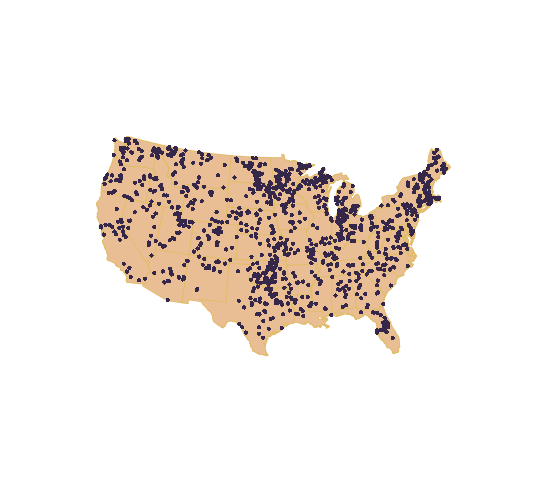
\includegraphics{./manuscript_files/figure-latex/nlaMap-1.png}
\caption{Map of the distribution of National Lakes Assesment Sampling
locations\label{fig:nlaMap}}
\end{figure}

\newpage

\begin{figure}[htbp]
\centering
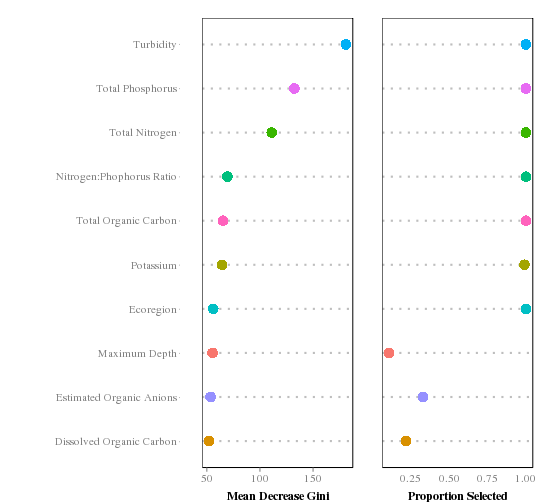
\includegraphics{./manuscript_files/figure-latex/Importance_Model1-1.png}
\caption{Importance plot for Model 1\label{fig:Importance_Model1}}
\end{figure}

\newpage

\begin{figure}[htbp]
\centering
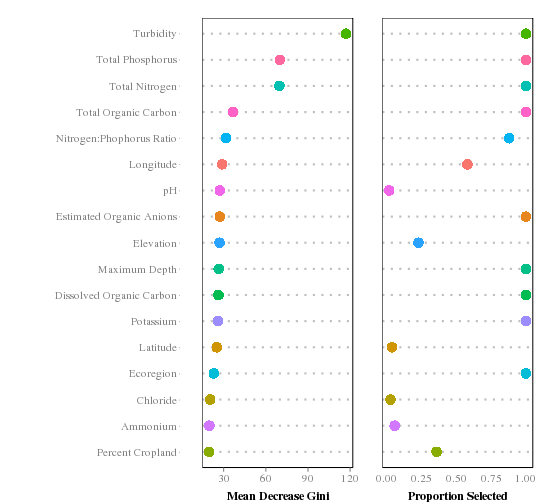
\includegraphics{./manuscript_files/figure-latex/Importance_Model2-1.png}
\caption{Importance plot for Model 2\label{fig:Importance_Model2}}
\end{figure}

\newpage

\begin{figure}[htbp]
\centering
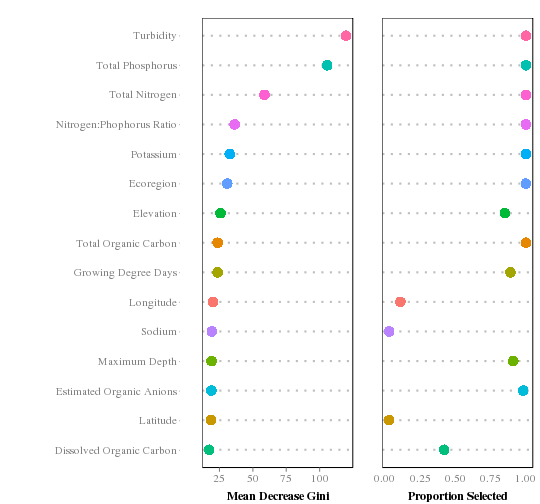
\includegraphics{./manuscript_files/figure-latex/Importance_Model3-1.png}
\caption{Importance plot for Model 3\label{fig:Importance_Model3}}
\end{figure}

\newpage

\begin{figure}[htbp]
\centering
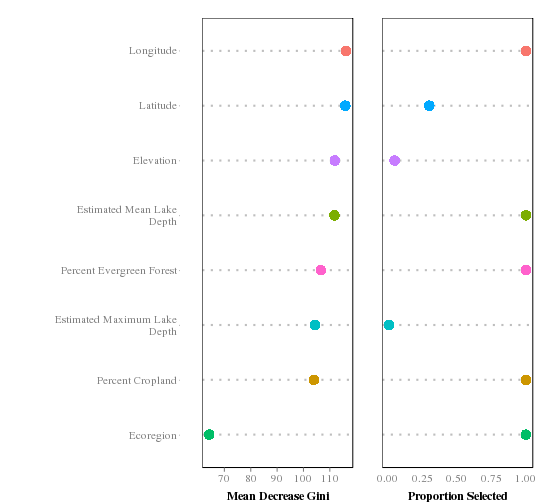
\includegraphics{./manuscript_files/figure-latex/Importance_Model4-1.png}
\caption{Importance plot for Model 4\label{fig:Importance_Model4}}
\end{figure}

\newpage

\begin{figure}[htbp]
\centering
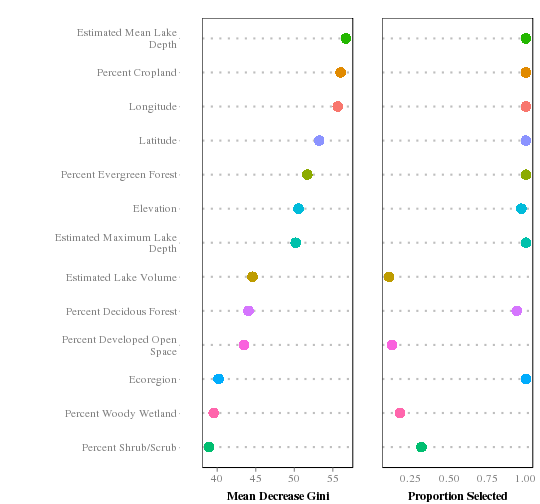
\includegraphics{./manuscript_files/figure-latex/Importance_Model5-1.png}
\caption{Importance plot for Model 5\label{fig:Importance_Model5}}
\end{figure}

\newpage

\begin{figure}[htbp]
\centering
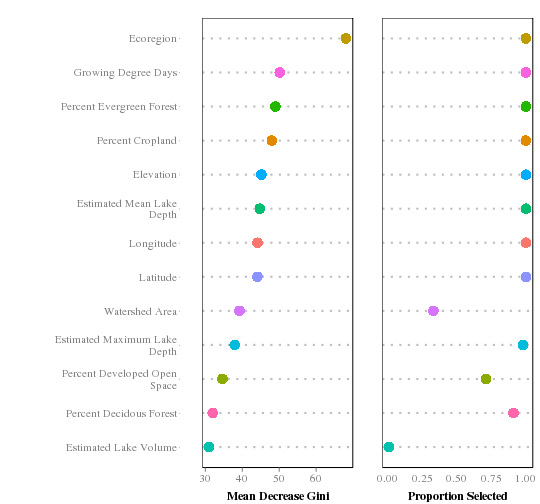
\includegraphics{./manuscript_files/figure-latex/Importance_Model6-1.png}
\caption{Importance plot for Model 6\label{fig:Importance_Model6}}
\end{figure}

\newpage

\begin{figure}[htbp]
\centering
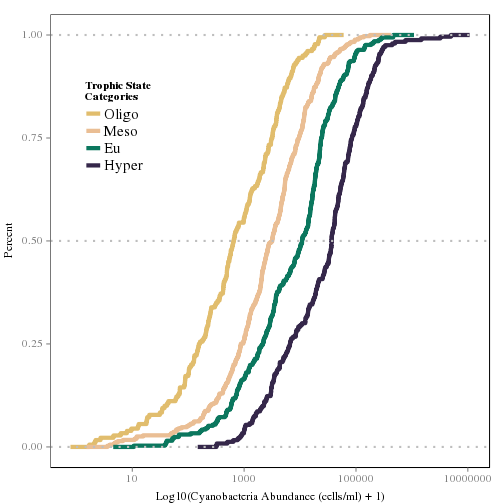
\includegraphics{./manuscript_files/figure-latex/ts_4_cyano_cdf-1.png}
\caption{Cumulative distribution function of cyanobacetria abundance for
4 trophic state classes\label{fig:ts_4_cyano_cdf}}
\end{figure}

\newpage

\begin{figure}[htbp]
\centering
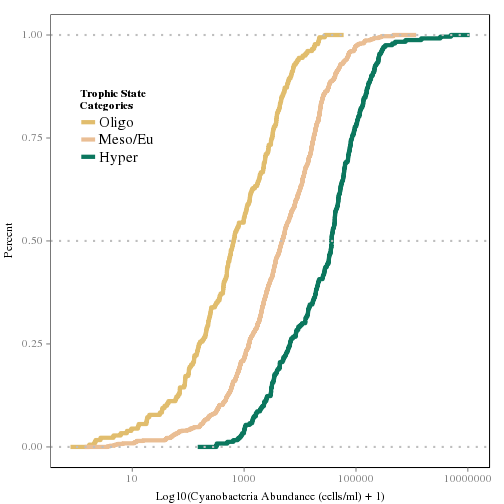
\includegraphics{./manuscript_files/figure-latex/ts_3_cyano_cdf-1.png}
\caption{Cumulative distribution function of cyanobacetria abundance for
3 trophic state classes\label{fig:ts_3_cyano_cdf}}
\end{figure}

\newpage

\begin{figure}[htbp]
\centering
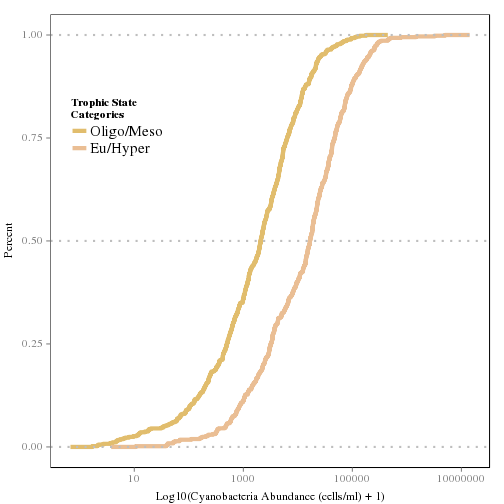
\includegraphics{./manuscript_files/figure-latex/ts_2_cyano_cdf-1.png}
\caption{Cumulative distribution function of cyanobacetria abundance for
2 trophic state classes\label{fig:ts_2_cyano_cdf}}
\end{figure}

\newpage

\begin{figure}[htbp]
\centering
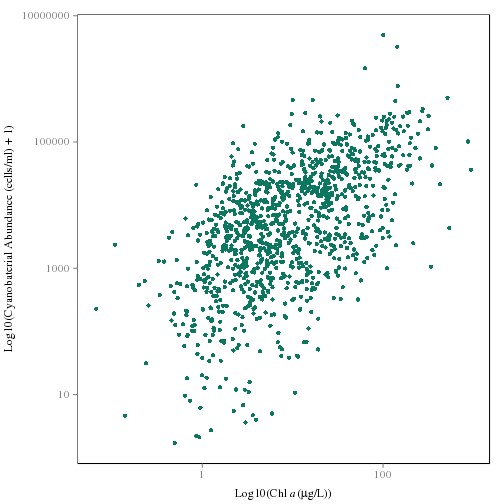
\includegraphics{./manuscript_files/figure-latex/scatterplot-1.png}
\caption{Cholorphyll \emph{a} and cyanobacteria abundance
scatterplot\label{fig:scatterplot}}
\end{figure}

\newpage

\begin{figure}[htbp]
\centering
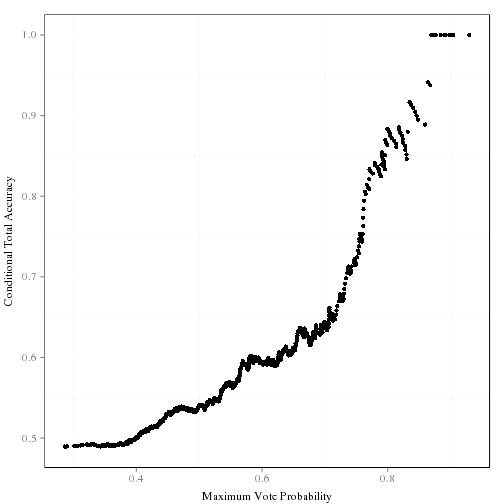
\includegraphics{./manuscript_files/figure-latex/condProbFig-1.png}
\caption{Comparison of certainity of trophic state prediction and total
accuracy\label{fig:condProbFig}}
\end{figure}

\newpage

\section{Tables}\label{tables}

\begin{longtable}[c]{@{}llllr@{}}
\toprule\addlinespace
Trophic State (4) & Trophic State (3) & Trophic State (2) & Cut-off & n
\\\addlinespace
\midrule\endhead
oligo & oligo & oligo/meso & \textless{}= 0.2 & 198
\\\addlinespace
meso & meso/eu & oligo/meso & \textgreater{}2-7 & 362
\\\addlinespace
eu & meso/eu & eu/hyper & \textgreater{}7-30 & 337
\\\addlinespace
hyper & hyper & eu/hyper & \textgreater{}30 & 246
\\\addlinespace
\bottomrule
\addlinespace
\caption{Chlorophyll a based trophic state
cut-offs\label{tab:trophicStateTable}}
\end{longtable}

\newpage

\begin{longtable}[c]{@{}lr@{}}
\toprule\addlinespace
Variable & Percent
\\\addlinespace
\midrule\endhead
NPratio & 1.00
\\\addlinespace
NTL & 1.00
\\\addlinespace
PTL & 1.00
\\\addlinespace
TOC & 1.00
\\\addlinespace
TURB & 1.00
\\\addlinespace
WSA\_ECO9 & 1.00
\\\addlinespace
K & 0.99
\\\addlinespace
ORGION & 0.33
\\\addlinespace
DOC & 0.22
\\\addlinespace
DEPTHMAX & 0.11
\\\addlinespace
\bottomrule
\addlinespace
\caption{Variable selection results for Model
1\label{tab:VarSel_Model1}}
\end{longtable}

\newpage

\begin{longtable}[c]{@{}lllll@{}}
\toprule\addlinespace
Oligo & Meso & Eu & Hyper & class.error
\\\addlinespace
\midrule\endhead
135 & 58 & 4 & 1 & 0.32
\\\addlinespace
42 & 233 & 77 & 10 & 0.36
\\\addlinespace
2 & 66 & 222 & 46 & 0.34
\\\addlinespace
0 & 3 & 69 & 174 & 0.29
\\\addlinespace
\bottomrule
\addlinespace
\caption{Random Forest confusion matrix for Model
1\label{tab:Confusion_Model1}}
\end{longtable}

\newpage

\begin{longtable}[c]{@{}lr@{}}
\toprule\addlinespace
Variable & Percent
\\\addlinespace
\midrule\endhead
DEPTHMAX & 1.00
\\\addlinespace
DOC & 1.00
\\\addlinespace
K & 1.00
\\\addlinespace
NTL & 1.00
\\\addlinespace
ORGION & 1.00
\\\addlinespace
PTL & 1.00
\\\addlinespace
TOC & 1.00
\\\addlinespace
TURB & 1.00
\\\addlinespace
WSA\_ECO9 & 1.00
\\\addlinespace
NPratio & 0.88
\\\addlinespace
AlbersX & 0.58
\\\addlinespace
CropsPer\_3000m & 0.36
\\\addlinespace
ELEV\_PT & 0.23
\\\addlinespace
NH4 & 0.06
\\\addlinespace
AlbersY & 0.04
\\\addlinespace
CL & 0.03
\\\addlinespace
PH\_FIELD & 0.02
\\\addlinespace
\bottomrule
\addlinespace
\caption{Variable selection results for Model
2\label{tab:VarSel_Model2}}
\end{longtable}

\newpage

\begin{longtable}[c]{@{}llll@{}}
\toprule\addlinespace
Oligo & Meso/Eu & Hyper & class.error
\\\addlinespace
\midrule\endhead
122 & 74 & 0 & 0.38
\\\addlinespace
43 & 604 & 42 & 0.12
\\\addlinespace
0 & 72 & 173 & 0.29
\\\addlinespace
\bottomrule
\addlinespace
\caption{Random Forest confusion matrix for Model
2\label{tab:Confusion_Model2}}
\end{longtable}

\newpage

\begin{longtable}[c]{@{}lr@{}}
\toprule\addlinespace
Variable & Percent
\\\addlinespace
\midrule\endhead
K & 1.00
\\\addlinespace
NPratio & 1.00
\\\addlinespace
NTL & 1.00
\\\addlinespace
PTL & 1.00
\\\addlinespace
TOC & 1.00
\\\addlinespace
TURB & 1.00
\\\addlinespace
WSA\_ECO9 & 1.00
\\\addlinespace
ORGION & 0.98
\\\addlinespace
DEPTHMAX & 0.91
\\\addlinespace
DDs45 & 0.89
\\\addlinespace
ELEV\_PT & 0.85
\\\addlinespace
DOC & 0.42
\\\addlinespace
AlbersX & 0.11
\\\addlinespace
AlbersY & 0.03
\\\addlinespace
Na & 0.03
\\\addlinespace
\bottomrule
\addlinespace
\caption{Variable selection results for Model
3\label{tab:VarSel_Model3}}
\end{longtable}

\newpage

\begin{longtable}[c]{@{}lll@{}}
\toprule\addlinespace
Oligo/Meso & Eu/Hyper & class.error
\\\addlinespace
\midrule\endhead
485 & 75 & 0.13
\\\addlinespace
77 & 505 & 0.13
\\\addlinespace
\bottomrule
\addlinespace
\caption{Random Forest confusion matrix for Model
3\label{tab:Confusion_Model3}}
\end{longtable}

\newpage

\begin{longtable}[c]{@{}lr@{}}
\toprule\addlinespace
Variable & Percent
\\\addlinespace
\midrule\endhead
AlbersX & 1.00
\\\addlinespace
CropsPer\_3000m & 1.00
\\\addlinespace
EvergreenPer\_3000m & 1.00
\\\addlinespace
MeanDepthCorrect & 1.00
\\\addlinespace
WSA\_ECO9 & 1.00
\\\addlinespace
AlbersY & 0.30
\\\addlinespace
ELEV\_PT & 0.05
\\\addlinespace
MaxDepthCorrect & 0.01
\\\addlinespace
\bottomrule
\addlinespace
\caption{Variable selection results for Model
4\label{tab:VarSel_Model4}}
\end{longtable}

\newpage

\begin{longtable}[c]{@{}lllll@{}}
\toprule\addlinespace
Oligo & Meso & Eu & Hyper & class.error
\\\addlinespace
\midrule\endhead
94 & 72 & 28 & 2 & 0.52
\\\addlinespace
50 & 201 & 80 & 30 & 0.44
\\\addlinespace
21 & 110 & 131 & 73 & 0.61
\\\addlinespace
1 & 34 & 80 & 131 & 0.47
\\\addlinespace
\bottomrule
\addlinespace
\caption{Random Forest confusion matrix for Model
4\label{tab:Confusion_Model4}}
\end{longtable}

\newpage

\begin{longtable}[c]{@{}lr@{}}
\toprule\addlinespace
Variable & Percent
\\\addlinespace
\midrule\endhead
AlbersX & 1.00
\\\addlinespace
AlbersY & 1.00
\\\addlinespace
CropsPer\_3000m & 1.00
\\\addlinespace
EvergreenPer\_3000m & 1.00
\\\addlinespace
MaxDepthCorrect & 1.00
\\\addlinespace
MeanDepthCorrect & 1.00
\\\addlinespace
WSA\_ECO9 & 1.00
\\\addlinespace
ELEV\_PT & 0.97
\\\addlinespace
DeciduousPer\_3000m & 0.94
\\\addlinespace
ShrubPer\_3000m & 0.32
\\\addlinespace
WoodyWetPer\_3000m & 0.18
\\\addlinespace
DevOpenPer\_3000m & 0.13
\\\addlinespace
VolumeCorrect & 0.11
\\\addlinespace
\bottomrule
\addlinespace
\caption{Variable selection results for Model
5\label{tab:VarSel_Model5}}
\end{longtable}

\newpage

\begin{longtable}[c]{@{}llll@{}}
\toprule\addlinespace
Oligo & Meso/Eu & Hyper & class.error
\\\addlinespace
\midrule\endhead
80 & 115 & 1 & 0.59
\\\addlinespace
50 & 585 & 61 & 0.16
\\\addlinespace
0 & 142 & 104 & 0.58
\\\addlinespace
\bottomrule
\addlinespace
\caption{Random Forest confusion matrix for Model
5\label{tab:Confusion_Model5}}
\end{longtable}

\newpage

\begin{longtable}[c]{@{}lr@{}}
\toprule\addlinespace
Variable & Percent
\\\addlinespace
\midrule\endhead
AlbersX & 1.00
\\\addlinespace
AlbersY & 1.00
\\\addlinespace
CropsPer\_3000m & 1.00
\\\addlinespace
DDs45 & 1.00
\\\addlinespace
ELEV\_PT & 1.00
\\\addlinespace
EvergreenPer\_3000m & 1.00
\\\addlinespace
MeanDepthCorrect & 1.00
\\\addlinespace
WSA\_ECO9 & 1.00
\\\addlinespace
MaxDepthCorrect & 0.98
\\\addlinespace
DeciduousPer\_3000m & 0.91
\\\addlinespace
DevOpenPer\_3000m & 0.71
\\\addlinespace
BASINAREA & 0.33
\\\addlinespace
VolumeCorrect & 0.01
\\\addlinespace
\bottomrule
\addlinespace
\caption{Variable selection results for Model
6\label{tab:VarSel_Model6}}
\end{longtable}

\newpage

\begin{longtable}[c]{@{}lll@{}}
\toprule\addlinespace
Oligo/Meso & Eu/Hyper & class.error
\\\addlinespace
\midrule\endhead
428 & 129 & 0.23
\\\addlinespace
147 & 434 & 0.25
\\\addlinespace
\bottomrule
\addlinespace
\caption{Random forest confusion matrix for Model
6\label{tab:Confusion_Model6}}
\end{longtable}

\newpage

\begin{longtable}[c]{@{}rrrr@{}}
\toprule\addlinespace
Oligo & Meso & Eu & Hyper
\\\addlinespace
\midrule\endhead
0.8127741 & 0.1858553 & 0.0013706 & 0
\\\addlinespace
\bottomrule
\addlinespace
\caption{Example Lake Random Forest Vote Results\label{tab:voteTable}}
\end{longtable}

\section*{References}\label{references}
\addcontentsline{toc}{section}{References}

Breiman, L. 2001. Random forests. Machine learning 45:5--32.

Carlson, R. E. 1977. A trophic state index for lakes. Limnology and
oceanography 22:361--369.

Carvalho, L., C. A. Miller (nee Ferguson), E. M. Scott, G. A. Codd, P.
S. Davies, and A. N. Tyler. 2011. Cyanobacterial blooms: Statistical
models describing risk factors for national-scale lake assessment and
lake management. Science of The Total Environment 409:5353--5358.

Cutler, D. R., T. C. Edwards Jr, K. H. Beard, A. Cutler, K. T. Hess, J.
Gibson, and J. J. Lawler. 2007. Random forests for classification in
ecology. Ecology 88:2783--2792.

Diaz-Uriarte, R. 2010. varSelRF: Variable selection using random
forests.

D{í}az-Uriarte, R., and S. A. De Andres. 2006. Gene selection and
classification of microarray data using random forest. BMC
bioinformatics 7:3.

Hollister, J. W. 2014. lakemorpho: Lake morphometry in r.

Hollister, J. W., W. B. Milstead, and M. A. Urrutia. 2011. Predicting
maximum lake depth from surrounding topography. PLoS ONE 6:e25764.

Hollister, J. W., H. A. Walker, and J. F. Paul. 2008. CProb: a
computational tool for conducting conditional probability analysis.
Journal of environmental quality 37:2392--2396.

Hollister, J., and W. B. Milstead. 2010. Using gIS to estimate lake
volume from limited data. Lake and Reservoir Management 26:194--199.

Homer, C., C. Huang, L. Yang, B. Wylie, and M. Coan. 2004. Development
of a 2001 national land-cover database for the united states.
Photogrammetric Engineering \& Remote Sensing 70:829--840.

Imboden, D., and R. G{ä}chter. 1978. A dynamic lake model for trophic
state prediction. Ecological modelling 4:77--98.

Jeff Hollister, B. M., and B. Kreakie. (n.d.). LakeTrophicModelling:
Package to reproduce hollister et al. (2014) modeling lake trophic
state: A data mining approach.

Jones, J., M. Knowlton, D. Obrecht, and E. Cook. 2004. Importance of
landscape variables and morphology on nutrients in missouri reservoirs.
Canadian Journal of Fisheries and Aquatic Sciences 61:1503--1512.

Jones, K. B., A. C. Neale, M. S. Nash, R. D. Van Remortel, J. D.
Wickham, K. H. Riitters, and R. V. O'Neill. 2001. Predicting nutrient
and sediment loadings to streams from landscape metrics: a multiple
watershed study from the united states mid-atlantic region. Landscape
Ecology 16:301--312.

Liaw, A., and M. Wiener. 2002. Classification and regression by
randomForest. R News 2:18--22.

Milstead, W. B., J. W. Hollister, R. B. Moore, and H. A. Walker. 2013.
Estimating summer nutrient concentrations in northeastern lakes from
sPARROW load predictions and modeled lake depth and volume. PloS one
8:e81457.

Paul, J. F., and M. E. McDonald. 2005. DEVELOPMENT oF eMPIRICAL,
gEOGRAPHICALLY sPECIFIC wATER qUALITY cRITERIA: A cONDITIONAL
pROBABILITY aNALYSIS aPPROACH1. Wiley Online Library.

Peters, J., B. D. Baets, N. E. Verhoest, R. Samson, S. Degroeve, P. D.
Becker, and W. Huybrechts. 2007. Random forests as a tool for
ecohydrological distribution modelling. Ecological Modelling
207:304--318.

Salas, H. J., and P. Martino. 1991. A simplified phosphorus trophic
state model for warm-water tropical lakes. Water research 25:341--350.

Seilheimer, T. S., P. L. Zimmerman, K. M. Stueve, and C. H. Perry. 2013.
Landscape-scale modeling of water quality in lake superior and lake
michigan watersheds: How useful are forest-based indicators? Journal of
Great Lakes Research 39:211--223.

Smith, V. H. 1998. Cultural eutrophication of inland, estuarine, and
coastal waters. Pages 7--49 \emph{in} Successes, limitations, and
frontiers in ecosystem science. Springer.

Smith, V. H., S. B. Joye, R. W. Howarth, and others. 2006.
Eutrophication of freshwater and marine ecosystems. Limnology and
Oceanography 51:351--355.

Smith, V. H., G. D. Tilman, and J. C. Nekola. 1999. Eutrophication:
impacts of excess nutrient inputs on freshwater, marine, and terrestrial
ecosystems. Environmental pollution 100:179--196.

USEPA. 2009. National lakes assessment: a collaborative survey of the
nation's lakes. ePA 841-r-09-001. Office of Water; Office of Research;
Development, US Environmental Protection Agency Washington, DC.

Xian, G., C. Homer, and J. Fry. 2009. Updating the 2001 national land
cover database land cover classification to 2006 by using landsat
imagery change detection methods. Remote Sensing of Environment
113:1133--1147.

\end{document}